\documentclass[a4paper,11pt]{article}
\usepackage[margin=1in]{geometry}
\usepackage{tikz,tkz-graph,graphicx}
\usepackage{xcolor}
\usetikzlibrary{arrows.meta,positioning,shapes}

\definecolor{lightOrange}{rgb}{0.9921875,0.890625,0.69921875}
\definecolor{darkOrange}{rgb}{0.96875,0.64453125,0.33203125}

\begin{document}

\section*{Picture}
\begin{figure}[h]
  \centering
  \includegraphics[width=0.7\textwidth]{./1.png}
\end{figure}

\section*{PDF}
\begin{figure}[th]
\centering
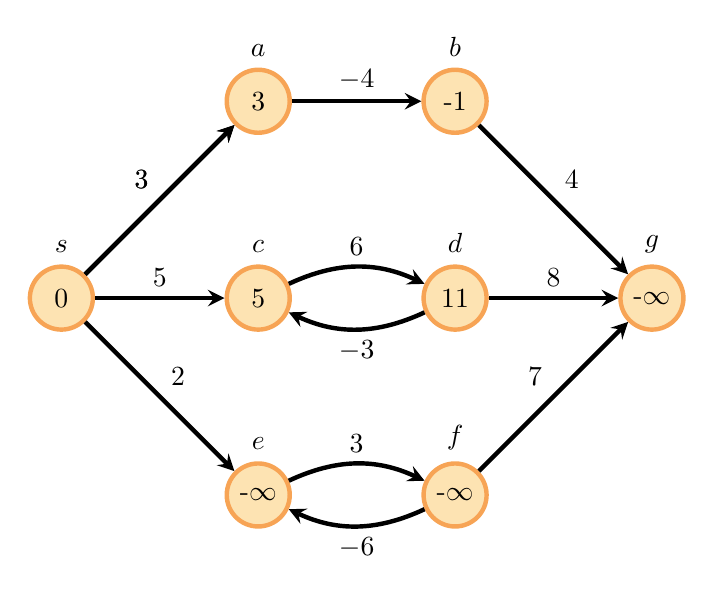
\begin{tikzpicture}[auto,main node/.style={circle,minimum size=8mm, draw=darkOrange,fill=lightOrange},scale=2,>=stealth,node distance=2.5cm,ultra thick]
    \node[main node, label=$c$] (c) [] {5};
    \node[main node, label=$s$] (s) [left of=c] {0};
    \node[main node, label=$a$] (a) [above of=c] {3};
    \node[main node, label=$e$] (e) [below of=c] {-$\infty$};
    \node[main node, label=$b$] (b) [right of=a] {-1};
    \node[main node, label=$d$] (d) [right of=c] {11};
    \node[main node, label=$g$] (g) [right of=d] {-$\infty$};
    \node[main node, label=$f$] (f) [right of=e] {-$\infty$};

    \path [->] (s) edge node {$3$} (a);
    \path [->] (s) edge node {$5$} (c);
    \path [->] (s) edge node {$2$} (e);
    \path [->] (a) edge node {$-4$} (b);
    \path [->] (b) edge node {$4$} (g);
    \path [->] (d) edge node {$8$} (g);
    \path [->] (f) edge node {$7$} (g);
    \path [->] (s) edge node {$3$} (a);
    \path [->] (c) edge[bend left=25] node{$6$} (d);
    \path [->] (d) edge[bend left=25] node{$-3$} (c);
    \path [->] (e) edge[bend left=25] node{$3$} (f);
    \path [->] (f) edge[bend left=25] node{$-6$} (e);
\end{tikzpicture}
\end{figure}

\end{document}
